\documentclass{article}
\usepackage{amsmath}
\usepackage{hyperref}
\usepackage{bookmark}
\usepackage{float} 
\usepackage{soul}
\usepackage{graphicx}
\usepackage{makeidx}
\usepackage[letterpaper, total={7.5in, 10in}]{geometry}

\makeindex

\begin{document}
\title{Electric Fields on Continuous Charge Distributions}
\author{Questions, Textbook; Answers, Elias Xu}
\date{February 4, 2025}
\maketitle
\setlength{\parindent}{0pt}

\section*{1}
\emph{In the figure below, two identical circular nonconducting rings are centered on the same line with their planes perpendicular to the line. Each ring has charge that is uniformly distributed along the circumference. The rings each produce electric fields at points along the line. The rings each produce electric fields at points along the line. For three situations, the charges on rings A and B are, respectively, \textbf{(1)} $q_0$ and $q_0$, \textbf{(2)} $-q_0$ and $-q_0$, \textbf{(3)} $-q_0$ and $q_0$. Rank the situations according to magnitude of the net electric field at \textbf{a} point $P_1$ midway between the rings, $P_2$  at the center of ring B, and \textbf{(c)} point $P_3$ to the right of ring B, greatest first  }
\begin{figure}[H]
    \centering
    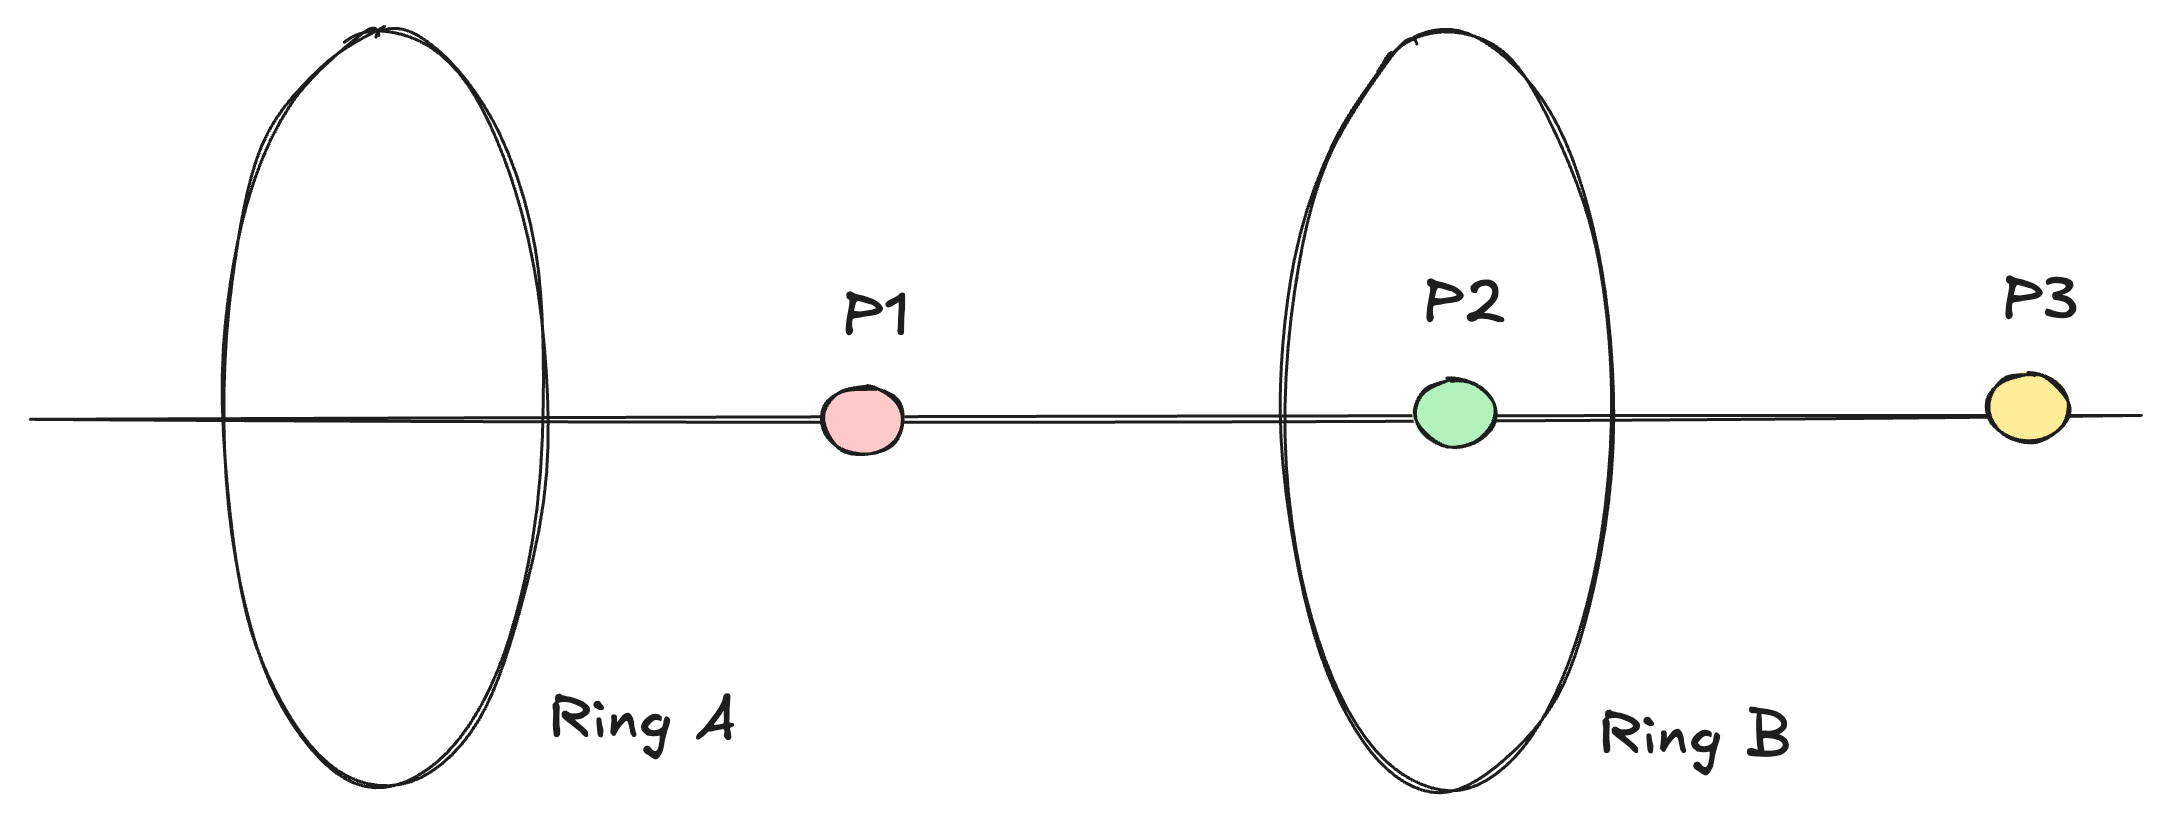
\includegraphics[width=0.9\textwidth]{figures/continuous_e_fields1.png}
\end{figure}
For point one in situations 3, it has two forces pulling in the same direction, 2 and 1 have the same forces pushing in opposite directions.\\
\textbf{(a)}: $\boxed{3 > 2 = 1}$ \\
For point two all of the sitations are equal because for each one there is only the force from ring 1 applied for each situation.\\
\textbf{(b)}: $\boxed{1 = 2 =3}$ \\
For point 3, one and two have both rings forces pointing in the same direction, the opposite happens in situation 3 \\
\textbf{(c)}: $\boxed{1 = 2 > 3}$


\section*{2} 
\emph{The diagram shows two concentric rings, or radii R and R' = 3.00R, that lie on the same plane. Point P lies on the central z axis, at distance D = 2.00 R from the center of the rings. the smaller ring has uniformly distributed charge +Q. In terms of Q, what is the uniformly distributed charge on the larger ring if the net eletric field is zero?}
\begin{figure}[H]
    \centering
    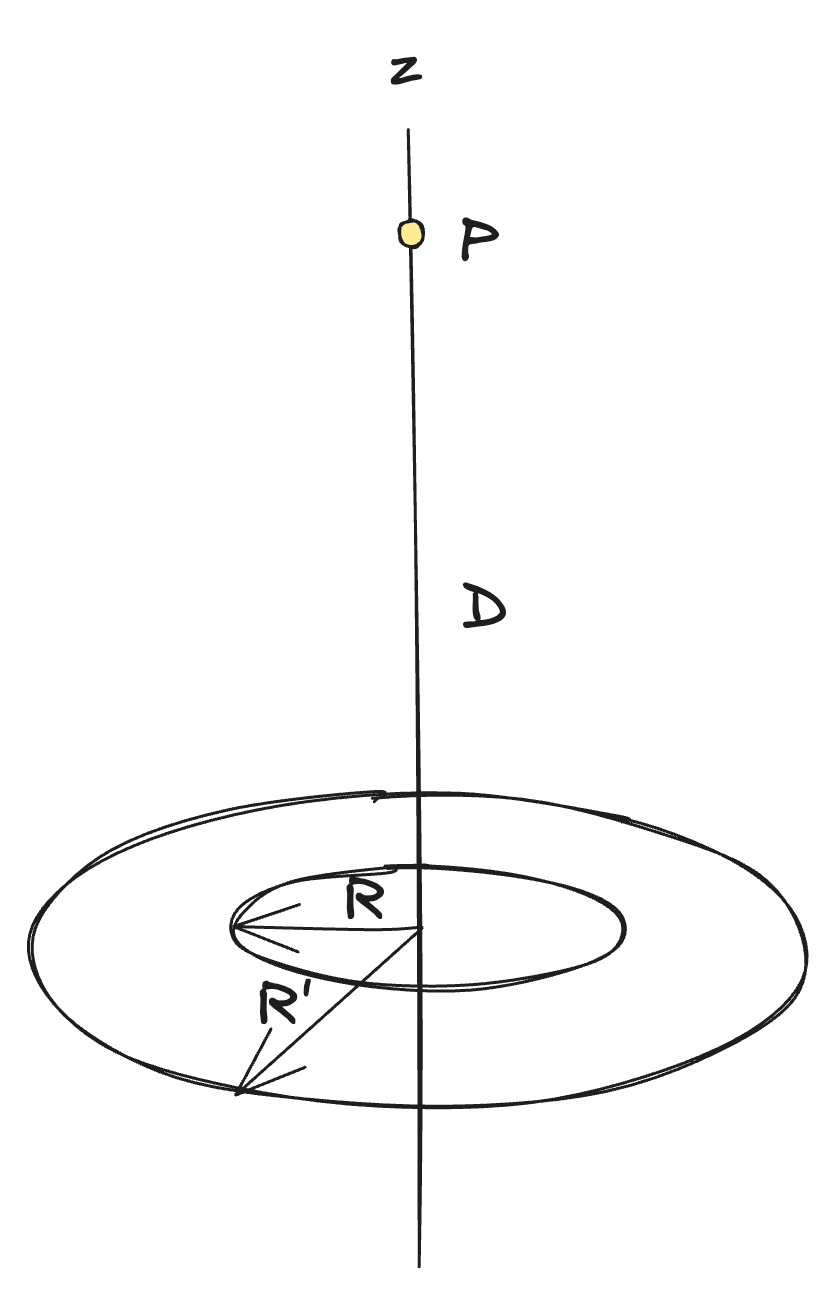
\includegraphics[width=0.2\textwidth]{figures/continuous_e_fields2.png}
\end{figure}
To solve, just do some bashing:
$$0 = \frac{Q D}{4 \pi\epsilon_0 (D^2 + R^2)^{\frac{3}{2}}} - \frac{Q' D}{4\pi\epsilon_0 (D^2 + R^{'2})^{\frac{3}{2}}}$$
$$\frac{Q'}{(D^2 + R'^2)^{\frac{3}{2}}} = \frac{Q}{(D^2 + R^2)^{\frac{3}{2}}}$$
$$Q' = \frac{(D^2 + R'^2)^{\frac{3}{2}}}{(D^2 + R^2)^{\frac{3}{2}}} Q = \boxed{-\sqrt{\frac{13^3}{5^3}} Q}$$

\end{document}